
\begin{figure}
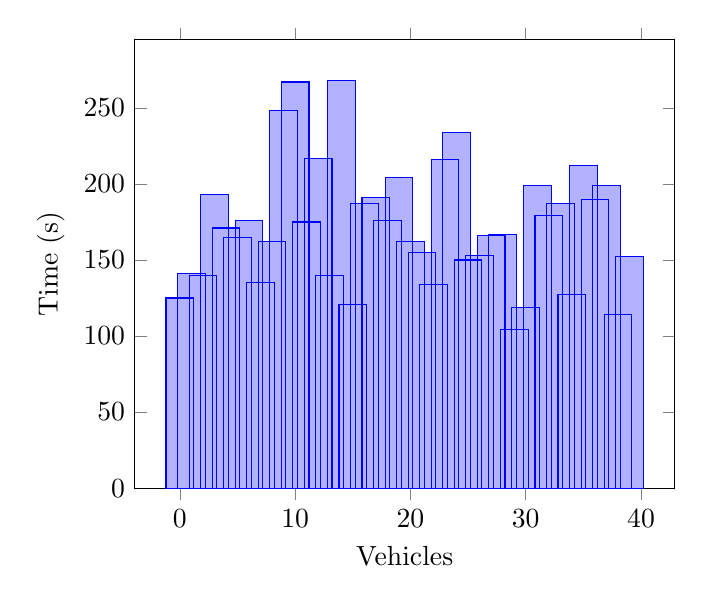
\begin{tikzpicture}
\begin{axis}[
legend style={anchor=west},
xlabel=Vehicles,
ylabel=Time (s),
ymin=0,
ybar,
]
\addplot coordinates {
(0, 125)
(1, 141)
(2, 140)
(3, 193)
(4, 171)
(5, 165)
(6, 176)
(7, 135)
(8, 162)
(9, 248)
(10, 267)
(11, 175)
(12, 217)
(13, 140)
(14, 268)
(15, 121)
(16, 187)
(17, 191)
(18, 176)
(19, 204)
(20, 162)
(21, 155)
(22, 134)
(23, 216)
(24, 234)
(25, 150)
(26, 153)
(27, 166)
(28, 167)
(29, 104)
(30, 119)
(31, 199)
(32, 179)
(33, 187)
(34, 127)
(35, 212)
(36, 190)
(37, 199)
(38, 114)
(39, 152)
};

\end{axis}
\end{tikzpicture}
\label{tik:100:2_O, 2_O.-60, 4_S, 5_S, 5_S.-30, 7_S, 7_S.-25, 11_S, 11_S.-50, 13_S, 15_N, 17_S, 17_S.-60, 18_S}
\caption{100 percent diving with GSC on route $2_O, 2_O.-60, 4_S, 5_S, 5_S.-30, 7_S, 7_S.-25, 11_S, 11_S.-50, 13_S, 15_N, 17_S, 17_S.-60, 18_S$}
\end{figure}
